% !TEX root = ../thesis.tex

\chapter{Neural network training data}
\label{chap:neural-network-data}

Over their relatively brief existance, neural networks have been shown to perform increasingly impressive tasks (e.g.  \cite{openai2019dota}, \cite{openai2023gpt4}, 
and many more). However, they learn by example. The performance of a neural network is directly linked to the input data it receives during training. If the 
training data is not an accurate example of real world information a network later operates on, insight gained from it is at best an approximation, and at worst
completely randomly generated data. 

As such, it is not a question \textit{if} some neural network architecture can learn to identify an extensive air shower from WCD data, but rather which 
implementation, fed with which information, does. For this purpose, this chapter explains the procedure with which training data is generated. As stated above, this
must occur with a focus on being representative of data actually measured in the SD array. The elected approach to create time traces is modularized. The structure
of this chapter reflects this. First, general comments about the characteristics of background data (i.e. the WCD detector response in the absence of an extensive 
air shower) are made in \autoref{sec:background-dataset}. Next, the process to extract signal originating from CRs is detailed in \autoref{sec:signal-dataset}.
Lastly, building the time trace from the aforementioned modules and drawing samples from it for a neural network to train on is done in 
\autoref{sec:sliding-window-analysis}.

\section{Background dataset}
\label{sec:background-dataset}

While a flux of partices causes elevated ADC levels in both the HG and LG channels of a WCD PMT during a shower event, the lack of such a phenomenon does not imply 
the readout information is uniformly flat. Instead, it hovers around the channels' baseline (c.f. \autoref{sec:surface-detector}) with occasional spikes upwards 
due to low-energy particles impinging on the detector. Coupled with electronic noise from the many digital components in the UUB, this constitutes the data that is 
collected inbetween air shower events.

\subsection{Accidental muons}
\label{ssec:accidental-muons}

Most low-energy background particles present in the detector are muons. These are produced in the upper atmosphere during cascading processes analog to 
\autoref{chap:physical-background}. Due to the low primary energy the electromagnetic component of the shower is thermalized before it reaches surface level. The 
muonic component by itself does not contain enough information to enable an accurate reconstruction of primary energy and origin. This fact, coupled with the high
flux of events at lower energies ($\Upphi|_{E=\SI{100}{\giga\electronvolt}} \approx \SI[per-mode=power]{1}{\per\meter\per\second}$ \cite{boezio2000measurement}) 
make these events unsuitable for analysis. Stray muons, even though they originate from extensive air showers, must consequently be considered background events.

The rate at which such particles traverse a WCD tank is $f_\text{Acc.}\approx\SI{4.665}{\kilo\hertz}$ \cite{DavidInjectionFrequency}. Their arrival time is 
Poisson-distributed. This implies that generally, one in 14 time traces contains signal from a low-energy background event. Coincidences of two accidental 
muons occur on a sub-percent level. Any higher order of coincidences is likely originating from a single air shower process. The typical signal recorded by the 
surface detector from a single muon is presented in \autoref{fig:muon-response}

\begin{figure}
	\centering
	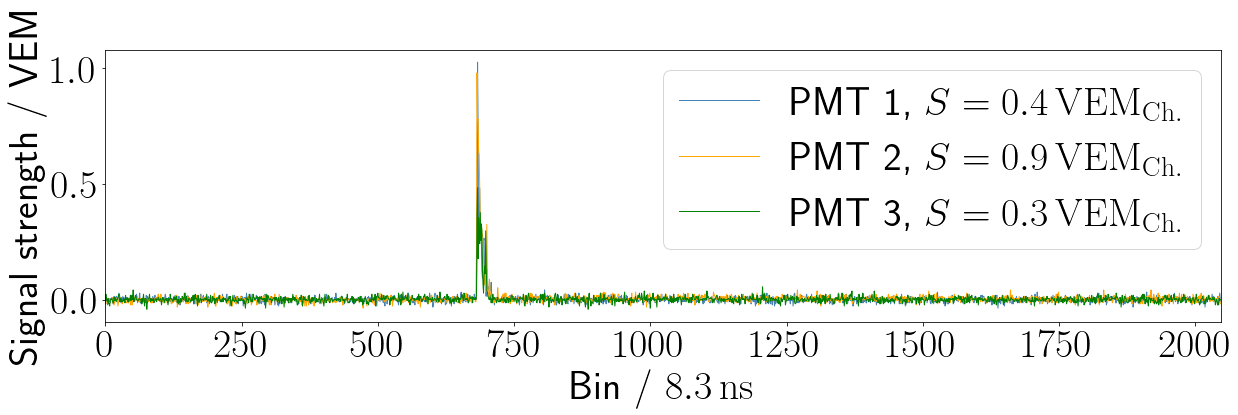
\includegraphics[width=0.8\textwidth]{./plots/muon_response.png}
	\caption{The simulated time trace from a single muon. The maximum peak of the time trace corresponds roughly to \SI{1}{\Peak}, wheras the integrated signal 
    $S$ per PMT sums up to \SI{1}{\Charge}.}
	\label{fig:muon-response}
\end{figure}

\subsection{Electronic noise}
\label{ssec:electronic-noise}

Electronic noise is the umbrella term given to the distortions that some signal is subject to during digital readout. Such noise can have many different origins.
An illustrative example is given by the \textbf{L}aser \textbf{I}nterferometer \textbf{G}ravitational wave \textbf{O}bservatory, which excludes the \SI{60}{\hertz}
band and its' harmonics from analysis. This is owed to the fact that the DC frequency standard in the United States introduces systematic uncertainties in the
detector \cite{martynov2016sensitivity}. In the electronics of Pierre Augers' SD array, electronic noise is assumed to be Gaussian. That is to say that the \ADC 
values of a time trace that was measured while no particle produced signal in the tank are normally distributed around the baseline. The standard deviation can be 
estimated from monitoring data, as is shown in \autoref{fig:standard-deviation-baseline}. \todo{make this plot}

\begin{figure}
	\centering
	\includegraphics[width=0.8\textwidth]{./plots/standard_deviation_baseline.png}
	\caption{ .}
	\label{fig:standard-deviation-baseline}
\end{figure}

\subsection{Random traces}
\label{ssec:random-traces}

Both above mentioned phenomena can be simulated, and the simulation results used as background training data for the neural networks discussed in the next chapter.
A more accurate method, and the approach elected for this work is to utilize directly measured data from the field. Thanks to the work of David Nitz, there exist
collections of so called random traces that were gathered by forcing DAQ readout via a manually set trigger. In particular, 

\subsubsection{Characteristics}
\label{ssec:random-trace-characteristics}



\subsubsection{Calibration}
\label{ssec:random-trace-calibration}

\todo{citing?}
\todo{spectral density}

\section{Signal dataset}
\label{sec:signal-dataset}



\section{Trace building \& Sliding window analysis}
\label{sec:sliding-window-analysis}
